\documentclass[12pt, letterpaper]{article}
\usepackage{setspace}
\usepackage{subcaption}
\usepackage[font={small,it}]{caption}\usepackage{graphicx}
\usepackage{array}
\usepackage{longtable}
\usepackage{quotes}
\usepackage{amsmath}
\usepackage{hyperref}
\usepackage[skip=10pt plus1pt, indent=40pt]{parskip}

% set reference files
\usepackage{biblatex}
\addbibresource{references.bib}

% set margins
\usepackage{geometry}
\geometry{margin=1in}

% Remove paragraph indentation
\setlength{\parindent}{0pt}


\graphicspath{{./figs/}{c:/Users/Zayan/Documents/code/personal_repos/neural_nets/ECE_8770/project_2/results}}
\onehalfspacing

\begin{document}

\begin{titlepage}
    \begin{center}

        \vspace*{1cm}

        \Large
        \textbf{ECE 8870 Project 2}

        \vspace{0.5cm}
        \textbf{Qazi Zarif Ul Islam}

        Pawprint: qzic2d

        \large

        \vspace{0.8cm}
        % \includegraphics[width=0.4\textwidth]{figs/Screenshot 2023-09-28 011032.png}

        University of Missouri-columbia \\
        04/21/2024
        
    \end{center}
\end{titlepage}

\section{Technical Description}

In this project, an RNN and an LSTM were implemented using pytorch.
The broader goal of this project was to understand the working principles of
RNNs and LSTMs and gain a comparative understanding of the two neural network
architectures. 

In the following sections, first the basic components of an RNN and an LSTM 
are introduced as well as an explanation of how backpropagation occurs in an 
RNN. This explanation will be more qualitative than mathematically rigorous. 
A more extensive treatment of backpropagation in RNNs can be found in ---. After that, the experiments and results shall be demonstrated and discussed before
a final conclustion section that talks about what more can be done to understand
RNNs and LSTMs and the deficiencies of this project.

The code is available at : \url{https://github.com/Murdock135/neural-nets-at-mizzou/tree/main/ECE_8770/project_2}

\subsection{Recurrent Neural Networks}

Recurrent Neural Networks are neural neural networks that store the 
hidden layer's output at the current time step so that it can influence
the output of the hidden layer at the next time step. Qualitatively,
this is commonly thought of as information being passed to the next time
step. Figure \ref{fig: rnns v1} shows this in two forms. On the left the 
rnn is said to be in "rolled"(in time) form whereas on the right is is said to be 
in "unrolled"(in time) form. The figure tells us that the rnn can be seen as a "feedback"
network of sorts where the output of the hidden layer $h_t$ is passed back to the hidden layer.
The left picture fails to capture that $h_t$ is passed to the next time step. The unrolled 
version captures this well. On the other hand, the rolled version captures a very crucial 
fact; that throughout the hidden layers at different time steps, \textit{there is only 
one weight matrix}, shared throughout the entire RNN at all time steps. Figure \ref{rnns v2} explicitly
illustrates this.

\begin{figure}[htpb]
    \centering
    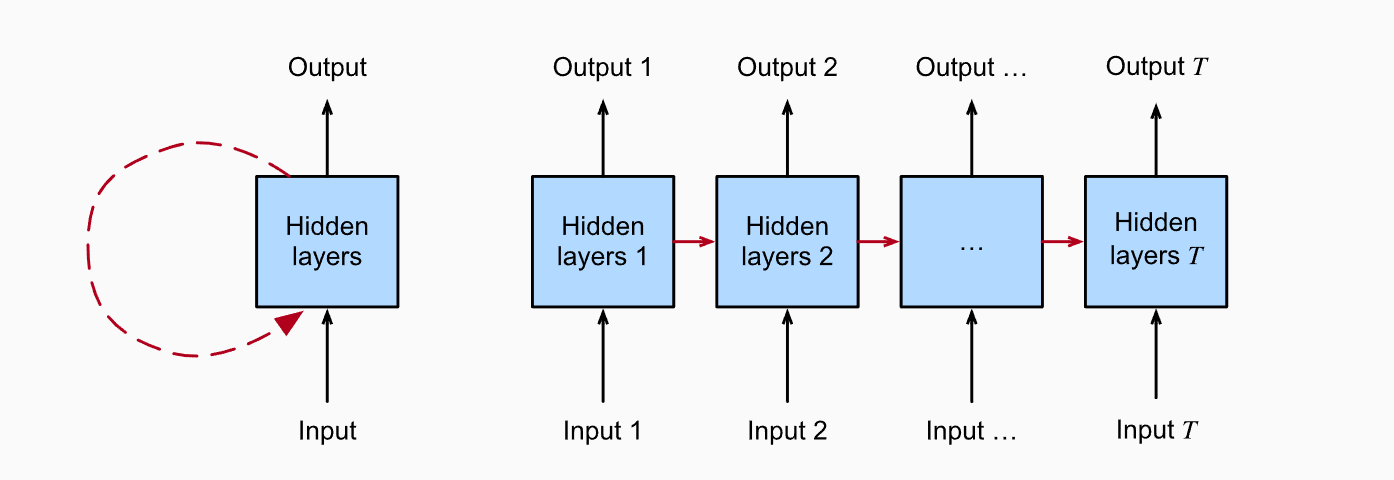
\includegraphics[width=0.8\textwidth]{d2l_ai_rnn_v1.png}
    \caption{\cite{zhang2023dive}: On the left recurrent connections are depicted via cyclic edges. 
    On the right, we unfold the RNN over time steps. Here, recurrent edges span 
    adjacent time steps, while conventional connections are computed synchronously}
    \label{fig: rnns v1}
\end{figure}

The shaded blue boxes are each a Multi-layer perceptron. The only caveat here is that in addition to the
inputs of the "current time step" $x_t$, it also recieves \textit{as} input, the weighted outputs of 
the previous hidden layer $h_{t-1}$. Thus, the input to the current hidden layer is expressed as a 
concatenation $[h_{t-1};\;x_t]$. Thus the equations defining the RNN are,

\begin{align}
    h_t = \phi(W_{hh} h_{t-1} + W_{xh} x_t + b_h)
    \label{eqn: h_t rnn}
\end{align}

\begin{equation}
    o_t = W_o h_t + b_o
    \label{eqn: o_t rnn}
\end{equation}

Where in equation \ref{eqn: h_t rnn}, $W_{hh}$ indicates \textbf{the weights going from the hidden layer at the previous time step to the 
hidden layer at the current time step}, $W_{xh}$ indicates \textbf{the weights going from the current 
inputs to the current hidden layer.} In equation \ref{eqn: o_t rnn} $W_o$ indicates \textbf{the weights going from
the hidden layer at the current time step to the output layer of the current time step.}

With these equations, the learning rule the RNN can be derived for any optimization algorithm e.g.
stochastic gradient descent, adaptive momentum, RMS prop, etc. The algorithms won't be discussed in 
this report but the gradients of the error wrt the learnable parameters are mentioned
in the next section, \textbf{backpropagation through time}.

\subsubsection{Backpropagation through time (Backpropagation for RNNs)}

\begin{figure}[htpb]
    \centering
    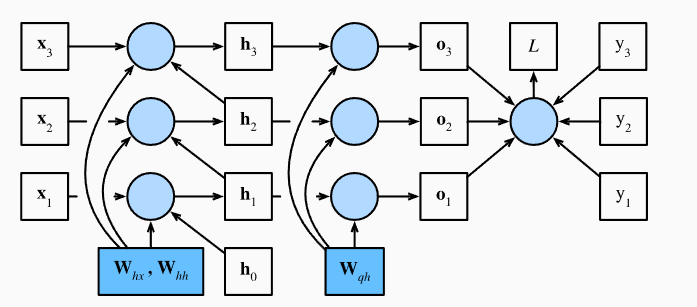
\includegraphics[width=0.8\textwidth]{d2l_ai_rnn_v2.png}
    \caption{\cite{zhang2023dive}: Computational graph showing dependencies for an RNN model 
    with three time steps. Boxes represent variables (not shaded) or parameters (shaded) and circles 
    represent operators.}
    \label{fig: rnns v2}
\end{figure}


For an RNN, the total loss is expressed as,

\begin{equation}
    \hat{L} = \frac{1}{T} \sum_{t=1}^{T} \ell(y_t, d_t) = \frac{1}{T} (l_1 + l_2 + ... + l_t ... + l_T)
    \label{eqn: total loss rnn}
\end{equation}

Where the small $l_t$'s indicate loss at a particular time step. The gradients of this total loss with respect
to the learnable parameters are, 

\begin{align}
    \frac{\partial l_t}{\partial w_h} &= \frac{\partial l_t}{\partial o_t}\frac{\partial o_t}{\partial h_t}\frac{\partial h_t}{\partial w_h} \label{eqn: rnn lt wrt w_h}\\
    \frac{\partial h_t}{\partial w_h} &= \frac{\partial h_t}{\partial w_h} + \sum_{i=1}^{t-1}\prod_{j-1=i}^{t} (\frac{\partial h_j}{\partial h_{j-1}}) \frac{\partial h_i}{\partial w_h}\label{eqn: rnn h_t wrt w_h}\\
    \frac{\partial L}{\partial W_{oh}} &= \sum_{t}^{T} \frac{\partial L}{\partial o_t} h_t \\
    \frac{\partial L}{\partial W_{hx}} &= \sum_{t}^{T} \frac{\partial L}{\partial h_t} x_t \\
    \frac{\partial L}{\partial w_h} &= \sum_{t}^T \frac{\partial l_t}{\partial o_t}\frac{\partial o_t}{\partial h_t}\frac{\partial h_t}{\partial w_h} \label{eqn: rnn total loss wrt w_h}
\end{align}

Where $w_h = [W_{hx};\; W_{hh}]$ is the concatenated weight matrix, 
$W_{oh}$ is the weight matrix from the hidden layer to the output layer, 
$W_{hx}$ is the weight matrix from the input layer to the hidden layer.

Observe \ref{eqn: rnn h_t wrt w_h}. Any gradient based algorithm would compute
this gradient and when it does, it has to recursively calculate the change of 
$h_j$ wrt $h_{j-1}$ and if the sequence is long, this product term will 
either be very large (if each gradient term $>1$) or be miniscule (if each gradient 
term $<1$). These two situations are called the \textit{exploding gradient} and 
the \textit{diminishing or vanishing gradient} problems, respectively. To solve
this issue, several techniques are used to truncate this product. \cite{zhang2023dive}
mentions two such techniques; \textit{(1) Regular truncation} and \textit{(2) Randomized
truncation.} The equations won't be derived in this report but an illustration of 
the three techniques is presented in fig \ref{fig: truncated_bptt}. In regular 
truncated BPTT, the sum is truncated after $\tau$ steps whereas in 
randomized BPTT, the initial sequences are split up into sub-sequences 
of "random" length (here, the length of the subsequences are cast as random
variables). \cite{tallec2017unbiasing}

\begin{figure}[htpb]
    \centering
    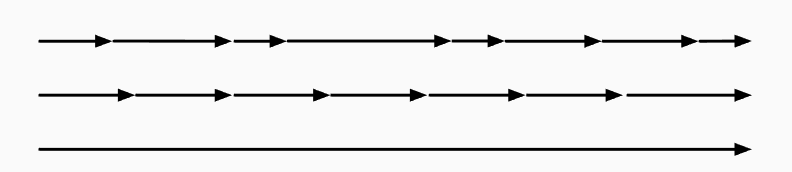
\includegraphics[width=0.8\textwidth]{techniques for truncated bptt.png}
    \caption{Comparing strategies for computing gradients in RNNs. From top to bottom: randomized truncation, regular truncation, and full computation.}
    \label{fig: truncated_bptt}
\end{figure}

\subsection{Long Short Term Memory nets (LSTMs)}

\begin{figure}[htpb]
    \centering
    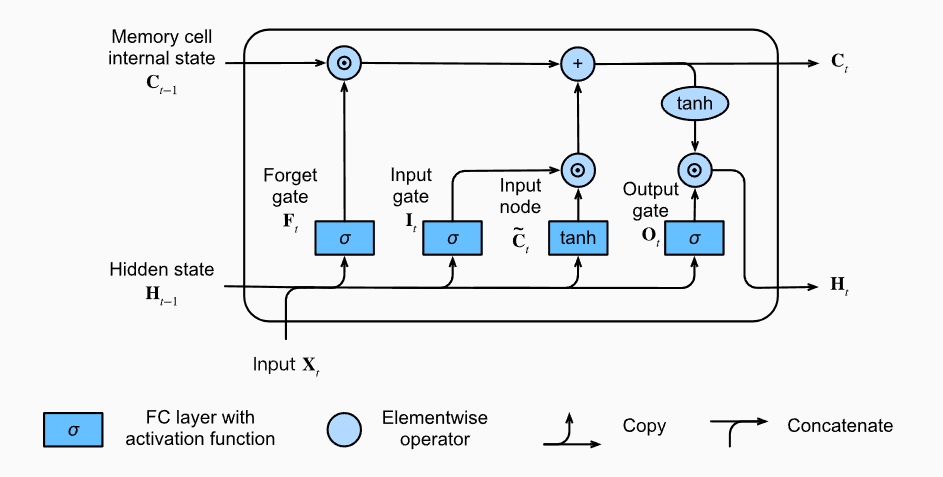
\includegraphics[width=0.8\textwidth]{lstms v1.png}
    \caption{lstms}
    \label{fig: lstms}
\end{figure}

LSTMs 

\subsection{RNN/LSTM configurations}

\section{Experiments and Results}


\subsection{Training details}

The following experiments were run on an NVIDIA CUDA RTX 3050 laptop GPU. The
machine has a total memory of 16 GigaBytes. Each experiment was run for 100 epochs.


\printbibliography

\end{document}